%%%%%%%%%%%%%%%%%%%%%%%%%%%%%%%%%%%%%%%%%
% Masters/Doctoral Thesis 
% LaTeX Template
% Version 2.5 (27/8/17)
%
% This template was downloaded from:
% http://www.LaTeXTemplates.com
% https://www.latextemplates.com/template/masters-doctoral-thesis
%
% Version 2.x major modifications by:
% Vel (vel@latextemplates.com)
%
% This template is based on a template by:
% Steve Gunn (http://users.ecs.soton.ac.uk/srg/softwaretools/document/templates/)
% Sunil Patel (http://www.sunilpatel.co.uk/thesis-template/)
%
% Template license:
% CC BY-NC-SA 3.0 (http://creativecommons.org/licenses/by-nc-sa/3.0/)
%
%%%%%%%%%%%%%%%%%%%%%%%%%%%%%%%%%%%%%%%%%

%----------------------------------------------------------------------------------------
%	PACKAGES AND OTHER DOCUMENT CONFIGURATIONS
%----------------------------------------------------------------------------------------

\documentclass[
11pt, % The default document font size, options: 10pt, 11pt, 12pt
oneside, % Two side (alternating margins) for binding by default, uncomment to switch to one side
english, % ngerman for German
singlespacing, % Single line spacing, alternatives: onehalfspacing or doublespacing
%draft, % Uncomment to enable draft mode (no pictures, no links, overfull hboxes indicated)
%nolistspacing, % If the document is onehalfspacing or doublespacing, uncomment this to set spacing in lists to single
%liststotoc, % Uncomment to add the list of figures/tables/etc to the table of contents
%toctotoc, % Uncomment to add the main table of contents to the table of contents
%parskip, % Uncomment to add space between paragraphs
%nohyperref, % Uncomment to not load the hyperref package
headsepline, % Uncomment to get a line under the header
%chapterinoneline, % Uncomment to place the chapter title next to the number on one line
%consistentlayout, % Uncomment to change the layout of the declaration, abstract and acknowledgements pages to match the default layout
]{MastersDoctoralThesis} % The class file specifying the document structure

\usepackage{lmodern}
\usepackage[utf8]{inputenc} % Required for inputting international characters
\usepackage[T1]{fontenc} % Output font encoding for international characters

% \usepackage{mathpazo} % Use the Palatino font by default

% \usepackage[backend=bibtex,style=authoryear,natbib=true]{biblatex} % Use the bibtex backend with the authoryear citation style (which resembles APA)
\usepackage[backend=biber,style=authoryear,natbib=true]{biblatex} % Use the bibtex backend with the authoryear citation style (which resembles APA)

\addbibresource{ressources.bib} % The filename of the bibliography

\usepackage[autostyle=true]{csquotes} % Required to generate language-dependent quotes in the bibliography

%custom packages:
\usepackage{defs}
\usepackage{tikzdefs}


%----------------------------------------------------------------------------------------
%	MARGIN SETTINGS
%----------------------------------------------------------------------------------------

\geometry{
	paper=a4paper, % Change to letterpaper for US letter
	inner=2.5cm, % Inner margin
	outer=3.8cm, % Outer margin
	bindingoffset=.5cm, % Binding offset
	top=1.5cm, % Top margin
	bottom=1.5cm, % Bottom margin
	%showframe, % Uncomment to show how the type block is set on the page
}

%----------------------------------------------------------------------------------------
%	THESIS INFORMATION
%----------------------------------------------------------------------------------------

% \thesistitle{Making use of the layer-wise statistics of a neural network for dataset-reconstruction} % Your thesis title, this is used in the title and abstract, print it elsewhere with \ttitle
% \thesistitle{What Information Stored in the Layer-Wise Statistics of a Neural Network Tell Us About the Dataset}
\thesistitle{What the Layer-Wise Statistics of a Neural Network Tell Us About the Dataset}
% \thesistitle{What Information About the Dataset Is Captured by the Layer-Wise Statistics of a Neural Network}
\supervisor{Prof. Dr. Gitta \textsc{Kutyniok}} % Your supervisor's name, this is used in the title page, print it elsewhere with \supname
\examiner{} % Your examiner's name, this is not currently used anywhere in the template, print it elsewhere with \examname
\degree{Bachelor of Science} % Your degree name, this is used in the title page and abstract, print it elsewhere with \degreename
\author{Kurt \textsc{Willis}} % Your name, this is used in the title page and abstract, print it elsewhere with \authorname
\addresses{} % Your address, this is not currently used anywhere in the template, print it elsewhere with \addressname

\subject{Mathematics, Computer Science} % Your subject area, this is not currently used anywhere in the template, print it elsewhere with \subjectname
\keywords{} % Keywords for your thesis, this is not currently used anywhere in the template, print it elsewhere with \keywordnames
\university{\href{https://www.tu.berlin/}{Technische Universität Berlin}} % Your university's name and URL, this is used in the title page and abstract, print it elsewhere with \univname
\department{\href{https://www.math.tu-berlin.de/menue/home/}{Institut für Mathematik}} % Your department's name and URL, this is used in the title page and abstract, print it elsewhere with \deptname
\group{\href{https://www.math.tu-berlin.de/fachgebiete_ag_modnumdiff/angewandtefunktionalanalysis/v_menue/afg/}{Fachgebiet Angewandte Funktionalanalysis}} % Your research group's name and URL, this is used in the title page, print it elsewhere with \groupname
\faculty{\href{https://www.naturwissenschaften.tu-berlin.de/menue/fakultaet_ii/}{Fakultät II }} % Your faculty's name and URL, this is used in the title page and abstract, print it elsewhere with \facname

\AtBeginDocument{
\hypersetup{pdftitle=\ttitle} % Set the PDF's title to your title
\hypersetup{pdfauthor=\authorname} % Set the PDF's author to your name
\hypersetup{pdfkeywords=\keywordnames} % Set the PDF's keywords to your keywords
}

\begin{document}

\frontmatter % Use roman page numbering style (i, ii, iii, iv...) for the pre-content pages

\pagestyle{plain} % Default to the plain heading style until the thesis style is called for the body content

%----------------------------------------------------------------------------------------
%	TITLE PAGE
%----------------------------------------------------------------------------------------

% \begin{titlepage}
% \begin{center}

% \vspace*{.06\textheight}
% {\scshape\LARGE \univname\par}\vspace{1.5cm} % University name
% \textsc{\Large Bachelor Thesis}\\[0.5cm] % Thesis type

% \HRule \\[0.4cm] % Horizontal line
% {\huge \bfseries \ttitle\par}\vspace{0.4cm} % Thesis title
% \HRule \\[1.5cm] % Horizontal line
 
% \begin{minipage}[t]{0.4\textwidth}
% \begin{flushleft} \large
% \emph{Author:}\\
% \href{https://willisk.github.io/}{\authorname} % Author name - remove the \href bracket to remove the link
% \end{flushleft}
% \end{minipage}
% \begin{minipage}[t]{0.4\textwidth}
% \begin{flushright} \large
% \emph{Supervisor:} \\
% \href{https://www.math.tu-berlin.de/fachgebiete_ag_modnumdiff/angewandtefunktionalanalysis/v_menue/mitarbeiter/kutyniok/v_menue/home/}{\supname} % Supervisor name - remove the \href bracket to remove the link  
% \end{flushright}
% \end{minipage}\\[3cm]
 
% \vfill

% \large \textit{A thesis submitted in fulfillment of the requirements\\ for the degree of \degreename}\\[0.3cm] % University requirement text
% \textit{in the}\\[0.4cm]
% \groupname\\\facname - \deptname\\[2cm] % Research group name and department name
 
% \vfill

% {\large \today}\\[4cm] % Date
% %\includegraphics{Logo} % University/department logo - uncomment to place it
 
% \vfill
% \end{center}
% \end{titlepage}

% %----------------------------------------------------------------------------------------
% %	DECLARATION PAGE
% %----------------------------------------------------------------------------------------

% \begin{declaration}
% \addchaptertocentry{\authorshipname} % Add the declaration to the table of contents

% \noindent Hiermit erkläre ich, dass ich die vorliegende Arbeit selbstständig und eigenhändig sowie
% ohne unerlaubte fremde Hilfe und ausschließlich unter Verwendung der aufgeführten Quellen
% und Hilfsmittel angefertigt habe. \\

% \noindent Berlin, \today
% \noindent \\[1cm]
% \rule[0.5em]{10em}{0.5pt} \\% This prints a line to write the date
% \authorname
% \end{declaration}

% \cleardoublepage

% %----------------------------------------------------------------------------------------
% %	QUOTATION PAGE
% %----------------------------------------------------------------------------------------

% %\vspace*{0.2\textheight}
% %
% %\noindent\enquote{\itshape Thanks to my solid academic training, today I can write hundreds of words on virtually any topic without possessing a shred of information, which is how I got a good job in journalism.}\bigbreak
% %
% %\hfill Dave Barry

% %----------------------------------------------------------------------------------------
% %	ABSTRACT PAGE
% %----------------------------------------------------------------------------------------

% \begin{abstract}
% \addchaptertocentry{\abstractname} % Add the abstract to the table of contents
% Thesis Abstract..
% % The Thesis Abstract is written here (and usually kept to just this page). The page is kept centered vertically so can expand into the blank space above the title too\ldots
% \end{abstract}

% %----------------------------------------------------------------------------------------
% %	ACKNOWLEDGEMENTS
% %----------------------------------------------------------------------------------------

% \begin{acknowledgements}
% \addchaptertocentry{\acknowledgementname} % Add the acknowledgements to the table of contents
% Acknowledgements..
% % The acknowledgments and the people to thank go here, don't forget to include your project advisor\ldots
% \end{acknowledgements}

% %----------------------------------------------------------------------------------------
% %	LIST OF CONTENTS/FIGURES/TABLES PAGES
% %----------------------------------------------------------------------------------------

% \tableofcontents % Prints the main table of contents

% \listoffigures % Prints the list of figures

% \listoftables % Prints the list of tables

%%----------------------------------------------------------------------------------------
%%	ABBREVIATIONS
%%----------------------------------------------------------------------------------------
%
%\begin{abbreviations}{ll} % Include a list of abbreviations (a table of two columns)
%
%\textbf{LAH} & \textbf{L}ist \textbf{A}bbreviations \textbf{H}ere\\
%\textbf{WSF} & \textbf{W}hat (it) \textbf{S}tands \textbf{F}or\\
%
%\end{abbreviations}
%
%%----------------------------------------------------------------------------------------
%%	PHYSICAL CONSTANTS/OTHER DEFINITIONS
%%----------------------------------------------------------------------------------------
%
%\begin{constants}{lr@{${}={}$}l} % The list of physical constants is a three column table
%
%% The \SI{}{} command is provided by the siunitx package, see its documentation for instructions on how to use it
%
%Speed of Light & $c_{0}$ & \SI{2.99792458e8}{\meter\per\second} (exact)\\
%%Constant Name & $Symbol$ & $Constant Value$ with units\\
%
%\end{constants}
%
%%----------------------------------------------------------------------------------------
%%	SYMBOLS
%%----------------------------------------------------------------------------------------
%
%\begin{symbols}{lll} % Include a list of Symbols (a three column table)
%
%$a$ & distance & \si{\meter} \\
%$P$ & power & \si{\watt} (\si{\joule\per\second}) \\
%%Symbol & Name & Unit \\
%
%\addlinespace % Gap to separate the Roman symbols from the Greek
%
%$\omega$ & angular frequency & \si{\radian} \\
%
%\end{symbols}
%
%%----------------------------------------------------------------------------------------
%%	DEDICATION
%%----------------------------------------------------------------------------------------
%
%\dedicatory{For/Dedicated to/To my\ldots} 

%----------------------------------------------------------------------------------------
%	THESIS CONTENT - CHAPTERS
%----------------------------------------------------------------------------------------

\mainmatter % Begin numeric (1,2,3...) page numbering

\pagestyle{thesis} % Return the page headers back to the "thesis" style

% Include the chapters of the thesis as separate files from the Chapters folder
% Uncomment the lines as you write the chapters


% 
% Chapter Template

\chapter{Background}
\label{chap:Background}

\section{Notation}

A \textbf{sample} $\vec z$ is an observation drawn from a joint distribution over the domain $\set Z = \set X \times \set Y$. 
It consists of a tuple $(\vec x, y)$ of an \textbf{input} $\vec x$ and a \textbf{label} $y$. 

\noindent
The input space $\set X$ typically is $\R^d$ and $\set Y$, the set of possible labels, is a set of integers $\{1, \dots, C\}$ for some whole number $C$, also known as the \textbf{number of classes}.

\noindent
A \textbf{bracket-notation} $\finiteset{\, \cdot \,}$ is used to denote the set of all \textit{finite non-empty} subsets.
$\set A = \{\vec z^{(i)}\}_{i=1}^{| \set A |} = \{(\vec x^{(i)}, y^{(i)})\}_{i=1}^{| \set A |} \in \finiteset{\set Z}$ is called a \textbf{data set}. $\set A $ contains \textit{i.i.d.} (independent and identically distributed) samples drawn from some distribution over $\set Z$.
A \textbf{sample batch} or simply \textbf{batch} is a \textit{non-empty} subset thereof.

\noindent
$\mean$ and $\var$ are used to denote the empirical sample mean and variance of the input.
\begin{align*}
    \mean ({\set A}) &= \frac 1 {\lvert \set A \rvert} \sum _{i=1}^{\lvert \set A \rvert} \vec x^{(i)} \; \in \set X \\
    \var ({\set A}) &= \frac 1 {\lvert \set A \rvert} \sum _{i=1}^{\lvert \set A \rvert} (\vec x^{(i)} - \mean ({\set A}))^2 \; \in \set X
\end{align*}


Given a sample batch $\set A$, the set $\set A|_c = \{(\vec x, y) \in \set A \mid y = c\}$ is the subset of $\set A$ \textbf{constrained} to samples of label $c$.


A \textbf{feature-mapping} is any function from input space $\R^d$ to $\R^m$ for some $m$.
A data set to data set mapping is obtained by applying a feature-mapping $\varphi$ to every input. Given a data set $\set A$, and a feature-mapping $\varphi$:
\[
    \varphi(\set A) := \{(\varphi(\vec x), y) \mid (\vec x, y) \in \set A\} \;
    \in \powerset Z
\]



\section{Loss function}
Given two data sets $\set A, \set B$, a \textbf{loss function} or \textbf{objective function} is a function $\loss : \finiteset{\set Z} \times \finiteset{Z} \to \R$ that is \textit{piecewise continuously differentiable} with regard to its inputs.
I. e. where 
\[
    \loss (\set A, \set B) = \loss (
    \,\{(\vec x^{(i)}_{\set A}, y^{(i)}_{\set A})\}_{i=0}^{|\set A|}\,,
    \,\{(\vec x^{(j)}_{\set B}, y^{(j)}_{\set B})\}_{j=0}^{|\set B|}\,) \,,
\]
is piecewise $\mathcal C^1$ with regard to $\vec x^{(i)}_{\set A}$
for all $i=1, \dots, |\set A|$, and $\vec x^{(j)}_{\set B}$ for all $j=1, \dots, |\set B|$.


For a given feature-mapping $\varphi$ that is piecewise $\mathcal C ^1$, it will be defined as follows.
% 
\[
    \loss _{\varphi} (\set A, \set B) = 
    \|\mean ({\varphi (\set A)}) - \mean ({\varphi (\set B)})\| +
    \|\var ({\varphi (\set A)}) - \var ({\varphi (\set B)})\|
\]
% 
A \textbf{class-dependent} loss can be obtained as follows:
\[
    \loss _\varphi ^{\mathcal C} (\set A, \set B) =
    \sum _{\substack{c = 1 \dots C \\ \set A|_c ,\, \set B|_c \neq \emptyset}} 
    \|\mean ({\varphi (\set A|_c)}) - \mean({\varphi (\set B|_c)})\|
    + \|\var ({\varphi (\set A|_c)}) - \var ({\varphi (\set B|_c)})\| 
\]

\subsection{Combinations}
% 
This notion can be extended to a collection of feature-maps [$\varphi_0, \dots, \varphi_n$].
A \textbf{collection} is used to refer to a \textit{non-empty finite} set.
\begin{align*}
    \loss_{[\varphi_1, \dots, \varphi_n]} (\set A, \set B) &= 
    \sum_{i=1}^n \loss_{\varphi_i} (\set A, \set B) \\
    %
    \loss_{[\varphi_1, \dots, \varphi_n]}^{\mathcal C} (\set A, \set B) &= 
    \sum_{i=1}^n \loss_{\varphi_i}^{\mathcal C} (\set A, \set B)
\end{align*}

% \chapter{Objective}
\label{chap:Objective}



%%%%%%%%%%%%%%%%%%%%%%%%%%%%%%%%%%%%%%%%%%%%%%%%
%%%%%%%%%  Section: Reconstruction   %%%%%%%%%%%
%%%%%%%%%%%%%%%%%%%%%%%%%%%%%%%%%%%%%%%%%%%%%%%%


\section{Reconstruction}
\label{sec:Reconstruction}

\begin{figure}[h]
    
% RECONSTRUCTION GRAPH
\begin{tikzpicture}[node distance=1cm and 1.7cm, auto]
%%Nodes

\node (D) [minimum height=3.5cm] {\distribution};
\node [above of= D, align=center, yshift=0.7cm] {data set \\ distribution};

\node (A) [node, right= 1cm of D, fill=red!7, yshift=1.5cm] {\textbf{target} \\ $\set A$};
\node (B) [node, right= 1cm of D, yshift=-1.5cm] {\textbf{original} \\ $\set B_\text{true}$};

\node (Bp) [node, right= of B, fill=blue!3] {perturbed \\ \textbf{source} \\ $\set B$}; %\\ $\set B = \delta (\set B_\text{true})$};
\node (Br) [node, right= of Bp, fill=blue!7] {\textbf{reconstructed} \\ $\rho (\set B)$};


%%Arrows
\draw [arrow, dashed, thin] (D) -- (A.190);
\draw [arrow, dashed, thin] (D) -- (B.170);


\draw [arrow, dashed, thin] (B) -- (Bp) 
node (Pert) [midway, function, dashed] {$\delta$};
\draw [linestart] (Bp) -- (Br) 
node (Rec) [midway, function, draw=blue, fill=white] {$\rho$};
\node [fill=white, below= 0cm of Rec] {\color{blue} \footnotesize optimize};
\node [fill=white, below= 0cm of Pert] {\footnotesize \textit{unknown}};


% \draw [dashed] (Rec) to [out=245, in=115] (Rec2);

\node (Net) [function, thick, minimum width= 1cm, above right= -0cm and 3.1cm of A] {$\varphi$};
\node [above right=-0.2cm and 0cm of Net] {\small feature-map};
\node (Loss) [function, thick, above= 1.5cm of Net] {Loss};

\pgfmathtruncatemacro{\OutL}{110}
\pgfmathtruncatemacro{\OutM}{95}
\pgfmathtruncatemacro{\OutR}{75}
\pgfmathtruncatemacro{\InL}{360-\OutL}
\pgfmathtruncatemacro{\InM}{360-\OutM}
\pgfmathtruncatemacro{\InR}{360-\OutR}

\draw [lineend] (Net.\InL) to [corner connect h=-0.7cm] (A.east);
\draw [arrowend] (Net.\OutL) to [out=90, in=270] (Loss.260);

\draw [line] (Net.\InM) to [rect connect h=-0.7cm] (Br.100);
\draw [arrowend] (Net.\OutM) to [out=90, in=270] (Loss.260);

\draw [line, blue] (Net.\InR) to [rect connect h=-0.4cm] (Br.80);
\draw [lineend, blue, connect v] (Net.\OutR) to (Loss.south);
\draw [arrowend, blue, connect h] (Br.192) to (Rec.east);

\path (Net.\OutL) -- node[midway, above= 0.15cm, sloped] {\small statistics}(Loss.260);
% \node [above= 0.5cm of Net, fill=white] {\footnotesize optimize};
% \draw [arrow, Mahogany, thin, bend left=20] (A) to node[near end, above] {\footnotesize trained} (Net);

\node [above= 1cm of B, yshift=-1.5cm] {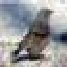
\includegraphics[]{figures/CIFAR10_example.pdf}};

\end{tikzpicture}




% % RECONSTRUCTION GRAPH
% \begin{tikzpicture}[node distance=1cm and 1.7cm, auto]
% %%Nodes

% \node (D) [minimum height=3.5cm] {\distribution};
% \node [above of= D, align=center, yshift=0.7cm] {data set \\ distribution};

% \node (A) [node, right= 1cm of D, fill=red!7, yshift=1.5cm] {\textbf{target} \\ $\set A$};
% \node (B) [node, right= 1cm of D, yshift=-1.5cm] {\textbf{original} \\ $\set B_\text{true}$}

% \node (Bp) [node, right= of B, fill=blue!3] {perturbed \\ \textbf{source} \\ $\set B$}; %\\ $\set B = \delta (\set B_\text{true})$};
% \node (Br) [node, right= of Bp, fill=blue!7] {\textbf{reconstructed} \\ $\rho (\set B)$};


% %%Arrows
% \draw [arrow, dashed, thin] (D) -- (A.190);
% \draw [arrow, dashed, thin] (D) -- (B.170);


% \draw [arrow, dashed, thin] (B) -- (Bp) 
% node (Pert) [midway, function, dashed] {$\delta$};
% \draw [linestart] (Bp) -- (Br) 
% node (Rec) [midway, function, draw=blue, fill=white] {$\rho$};
% \node [fill=white, below= 0cm of Rec] {\color{blue} \footnotesize optimize};
% \node [fill=white, below= 0cm of Pert] {\footnotesize \textit{unknown}};


% % \draw [dashed] (Rec) to [out=245, in=115] (Rec2);

% \node (Net) [function, thick, minimum width= 1cm, above right= -0cm and 3.1cm of A] {$\varphi$};
% \node [above right=-0.2cm and 0cm of Net] {\small feature-map};
% \node (Loss) [function, thick, above= 1.5cm of Net] {loss};

% \pgfmathtruncatemacro{\OutL}{110}
% \pgfmathtruncatemacro{\OutM}{95}
% \pgfmathtruncatemacro{\OutR}{75}
% \pgfmathtruncatemacro{\InL}{360-\OutL}
% \pgfmathtruncatemacro{\InM}{360-\OutM}
% \pgfmathtruncatemacro{\InR}{360-\OutR}

% \draw [lineend] (Net.\InL) to [corner connect h=-0.7cm] (A.east);
% \draw [arrowend] (Net.\OutL) to [out=90, in=270] (Loss.260);

% \draw [line] (Net.\InM) to [rect connect h=-0.7cm] (Br.100);
% \draw [arrowend] (Net.\OutM) to [out=90, in=270] (Loss.260);

% \draw [line, blue] (Net.\InR) to [rect connect h=-0.4cm] (Br.80);
% \draw [lineend, blue, connect v] (Net.\OutR) to (Loss.south);
% \draw [arrowend, blue, connect h] (Br.192) to (Rec.east);

% \path (Net.\OutL) -- node[midway, above= 0.15cm, sloped] {\small statistics}(Loss.260);
% % \node [above= 0.5cm of Net, fill=white] {\footnotesize optimize};
% % \draw [arrow, Mahogany, thin, bend left=20] (A) to node[near end, above] {\footnotesize trained} (Net);


% \end{tikzpicture}


    \caption{Overview}
    \centering
\end{figure}

This section describes the main objective of the task.
The goal is to learn an inverse transformation to the unknown $\delta$.
The way this is achieved is by maximizing similarity between the distributions of a source data set $\set B$
and a target data set $\set A$ in an appropriate feature-space $\phi$.
The goal of maximizing similarity in feature-space is addressed by formulating a loss function
that minimizes simple statistics, such as the mean and variance of the dataset.

Example application:
A neural network might be well adjusted to a target distribution, 
though under-perform when presented with samples that don't follow the original distribution
and exhibit different statistics to which the neural network was not adjusted to.
To combat this problem, a method for readjusting the inputs is introduced.
The basic idea is that the data is mapped to a feature-representation.
In this feature-space, simple statistics, such as the mean and variance are recorded
for both, a source data set $\set B$ and a target data set $\set A$.
Although, the source is first sent through a re-adjustment function $\rho$ that is
then tuned to minimize the similarity-loss of the two data sets.
This is done via a differentiable loss, or objective function that minimizes the difference in statistics.



\subsection{Problem Formulation}
Given: feature-map $\varphi$, target data set $\set A$ (or $\varphi(\set A)$ statistics), and a perturbed data set $\widetilde {\set B}$

\[
    \min_{\rho \in \mathcal{F}} \loss _\varphi (\set A, \rho(\widetilde{\set B})) \,,
\]
where $\mathcal F$ is a pre-defined set of functions.






%%%%%%%%%%%%%%%%%%%%%%%%%%%%%%%%%%%%%%%%%%%%%%%%
%%%%%%%%%%   Section: Inversion    %%%%%%%%%%%%%
%%%%%%%%%%%%%%%%%%%%%%%%%%%%%%%%%%%%%%%%%%%%%%%%


\section{Inversion}
\label{sec:Inversion}

\begin{tikzpicture}[node distance=1.3cm and 1.4cm, auto]

%%Nodes
\node (D) [minimum height=3.5cm] {\distribution};
\node [above of= D, align=center, yshift=0.2cm] {data set \\ distribution};

\node (N) [below= -0.5cm of D, minimum height=3.5cm] {\noise};
\node [above of= N] {random noise};

\node (B) [node, right= of N, fill=blue!7, draw=blue, thick] {\textbf{Source} \\ $\set B$};
\node (A) [node, right= of D, fill=red!7] {\textbf{target} \\ $\set A$};

\path (A) -- (B) node (Mid) [midway] {};
\node (Net) [function, thick, minimum width=1cm, right= of Mid, xshift=1.2cm] {$\varphi$};
\node [below right= 0.1cm and -1.2cm of Net] {\small feature-map};
\node (Loss) [function, thick, right= of Net] {loss};

%%Arrows
% \pgfmathtruncatemacro{\InL}{160}
% \pgfmathtruncatemacro{\InM}{175}
% \pgfmathtruncatemacro{\InR}{195}
% \pgfmathtruncatemacro{\OutL}{360-\InL}
% \pgfmathtruncatemacro{\OutM}{360-\InM}
% \pgfmathtruncatemacro{\OutR}{360-\InR}
\pgfmathtruncatemacro{\OutL}{20}
\pgfmathtruncatemacro{\OutM}{5}
\pgfmathtruncatemacro{\OutR}{-15}
\pgfmathtruncatemacro{\InL}{180-\OutL}
\pgfmathtruncatemacro{\InM}{180-\OutM}
\pgfmathtruncatemacro{\InR}{180-\OutR}

\draw [arrow, dashed, thin] (D) -- (A);
\draw [arrow, dashed, thin] (N) -- (B);

\draw [linestart] (A.east) to [rect connect v=1cm] (Net.\InL);
\draw [arrowend] (Net.\OutL) to[out=0, in=180]  (Loss.170);

\draw [linestart] (B.15) to [rect connect v=1cm] (Net.\InM);
\draw [arrowend] (Net.\OutM) to[out=0, in=180] (Loss.170);

\draw [arrowend, blue] (Net.\InR) to[out=180, in=0, rect connect v=-0.5cm] (B.-5);
\draw [lineend, blue, connect h] (Net.\OutR) to (Loss.west);
\node [below= 0cm of B, yshift=-0cm] {\color{blue} \footnotesize optimize};

\path (Net) -- (Loss) node [above=0.3cm, midway] {\small statistics};
% \draw [arrow, Mahogany, thin, bend left=30] (A.20) to [out=40, in=140] node[above, sloped] {\footnotesize trained} (Net);

\node [below= 0cm of A] {\fbox{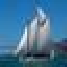
\includegraphics[]{figures/CIFAR10_example_3.pdf}}};

\end{tikzpicture}



The second part of this work is concerned about what kind of data may be recovered from 
having knowledge of the statistics of a data set.
For this task, the goal is to modify the source data set $\set B$ to more closely resemble
the target data set $\set A$ only given the statistics of data set $\set A$.
The source data set $\set B$ is in a first step, initialized by random noise.
Then, by performing gradient descent on the loss function, the source itself is optimized.



\subsection{Objective}
Given: $\varphi$, $\set A$ (or $\varphi(\set A)$ statistics), 
fixed size $n_{\set B}$, target labels $\{y^{(i)}\}_{i=1}^{n_{\set B}}$.
\[
    \min_{\set B \in \finiteset {\set Z}} \loss _\varphi (\set A, \set B) \comma{where} 
    \set B = \{(\vec x^{(i)}, y^{(i)})\}_{i=1}^{n_{\set B}}
\]
    


\subsection{Inversion Evaluation}
The result of the optimization process can be evaluated by calculating the accuracy obtained by $\Phi$. 
Though, since $\Phi$ was used in the optimization process, it will likely display heavy bias to what it believes is a correctly classified sample.
For this sake, another neural network $\Phi_{\text{ver}}$ can be employed, which has been separately trained on either $\set A$ or another data set. 

%Though, practice has shown that a very small portion of $\set A$ is only needed to obtain a close-enough guess at the true statistics of $\set A$.





\chapter{Experiments}
\label{chap:Experiments} 

\section{Methods}

The success of the reconstruction largely depends on the representation of the data
after the feature-map is applied.
Although, assuming that the data distribution of the data can be accurately described
by a mean and a variance is a strong assumption.
More sophisticated ways of modeling data distributions exist
\XXX{insert some}
, yet mean and variance were chosen due to their simplicity in evaluation and computing of the gradients.

The feature-map will ideally "disentangle" the data space to enable 
simple statistics to capture the complexity of the data set.

It is hypothesized that neural networks "disentangle" the input space in order to end up with an efficient feature-representation in its later layers.
(This becomes more apparent when one imagines that most neural networks must learn to classify by linearly separating its features obtained from the previous to last layer.)


For assessing the efficacy of the ability to capture the data distribution by
the statistics of the intermediary representations in a neural network,
several different mappings or collections of mappings will be compared. 

For every method there exists a class-dependent variant.
\subsection{Neural Network}

A \textbf{neural network} $\Phi$ is a function that maps an input $\vec x \in \R^d$ to a label $y$.
Normally, in classification tasks, where one hopes to assign a label to an input, the output of a neural network is a C-dimensional vector..
\XXX{maybe not, logit; DEF}. 
A \textbf{multi-layer perceptron} (MLP) is a special type of neural network. Throughout this work, when referring to a neural network, a multi-layer perceptron is meant. A MLP is a composition of functions $\Phi_i$, also called \textbf{layers} that successively act on the outputs $\vec h$ of the previous layer, called \textbf{activations} or \textbf{hidden states}. 
The last layer is referred to as the \textbf{logits-layer}. 
The predicted output label $\hat y$ is normally obtained by returning the index of the maximum value in the logits-layer, thus $\R^{\textnormal L} = \R^C$.
In a plain \textbf{fully-connected} neural network, the layers are each made up of an affine linear transformation and a non-linear activation function.

Formally, a fully-connected neural network of layer depth L is described as:

\[
    \Phi = \Phi_\text{L} \circ \ldots \circ \Phi_1
\]
\[
    \vec h_\ell = (\Phi_\ell \circ \ldots \circ \Phi_1) (\vec x) =
    \Phi_\ell(\vec h_{\ell-1}) \in \R^{d_\ell}
\]
$\Phi_\ell$ then, is a mapping from $\R^{d_{\ell-1}}$ to $\R^{d_\ell}$. 
The space of a hidden state $\vec h$ is called a \textbf{feature-space}.
The input $\vec x$ is also referred to as $\vec h_0$ and $\R^{d_0} := \R^d$.

\[
    \Phi_\ell(\vec h) = \sigma (\vec W \vec h + \vec b) \comma{where}
    \vec W \in \R^{d_\ell \times d_{\ell-1}} \comma{and}
    \vec b \in \R^{d_\ell}
\]
The affine linear transformation is made up of a \textbf{weight matrix} $\vec W$ and a \textbf{bias} $\vec b$.
The non-linear activation function $\sigma$ is often one of \textit{ReLU} (Rectified Linear Unit), \textit{tanh} or \textit{softmax}. The former two are mappings from $\R$ to $\R$ that are applied element-wise.




\subsection{Neural Network - last layer}

Given a neural network $\Phi$ of depth L..
A feature-mapping can be obtained by mapping inputs to the second-to-last layer.
Generally, this is seen as a layer with the best feature representation? source?


\[
    \varphi : \R^d \to \R^{d_\textnormal{L-1}} = (\Phi_\textnormal{L-1} \circ \dots \circ \Phi_1)
\]
\subsection{Neural Network - all layers}
All hidden states of the neural network are used to produce a collection of mappings [$\varphi_0, \dots, \varphi_\text{L}$].
\begin{alignat*}{2}
    \varphi_\ell &: \R^d \to \R^{d_\ell} &&= (\Phi_\ell \circ \dots \Phi_1) \quad
    \text{for $\ell = 1, \dots$, L - 1} \\
    \varphi_\textnormal{L} &: \R^d \to \R^d &&= \Id
\end{alignat*}





\subsection{Random Projections}
The method of projecting the input to the hidden representations of a neural network will be contrasted with taking $n$ random linear projections.
A random projection is a linear mapping $r: \R^d \to \R$
It is created by choosing a normalized random vector $\vec v \in S^{d-1} = \{\vec x \in \R^d : \|\vec x\| = 1\}$.
It is a simple linear projection on to the one-dimensional subspace defined by the vector $\vec v$.
\[
    r(\vec x) = \vec v ^\top \vec x
\]
By choosing a total of n random vectors $\{v_1, \dots, v_n\}$ one obtains a linear mapping $R: \R^d \to \R^n$:
\[
    R(\vec x) = \vec V \vec x =
    \begin{bmatrix}
        - \vec v_1 ^\top - \\
        \vdots \\
        - \vec v_n ^\top - \\
    \end{bmatrix}
    \vec x =
    \begin{bmatrix}
        \vec v_1 ^\top \vec x \\
        \vdots \\
        \vec v_n ^\top \vec x \\
    \end{bmatrix}
\]
%
The loss function $\loss_R$ stays as was defined before.
Though it might be more reasonable to have the projection centered around a more suitable position than to just project from the origin, in order to obtain better scaled values.
% 
\[
    R_{\vec o} (\vec x) = \vec V (\vec x - \vec o) \,,
\]
where $\vec o \in \R^d$ is the new origin of the projection. Although, practically one often works with normalized data anyhow..
The class-dependent variant can be modified to select an origin $\vec o_c$ for each class $c$.
% 
\begin{align*}
    \loss _R ^{\mathcal C} (\set A, \set B) &=
    \begin{aligned}[t]
        \sum _{\substack{c = 1 \dots C \\ \set A|_c ,\, \set B|_c \neq \emptyset}} 
        \|\mean ({R_{\vec o_c} (\set A|_c)}) - \mean ({R_{\vec o_c} (\set B|_c)}) \| \\
        {} + \|\var ({R_{\vec o_c} (\set A|_c)}) - \var ({R_{\vec o_c} (\set B|_c)}) \| 
    \end{aligned}
\end{align*}

The idea is to set the origin to be at the center of each class of the target data set $\set A$. $\vec o_c = \mean ({\set A|_c})$
This way we can ensure a balanced output..



\subsection{Random Projections ReLU}
To further explore the influence of the non-linear activation functions contained within the network,
one can combine the previous method with adding an activation function, in this case the ReLU.
% 
\[
    R_{\vec o}^+ (\vec x) = (\vec V (\vec x - \vec o))^+ \,,
\]
where $(\,\cdot\,)^+ :\R^n \to \R^n$ is the projection onto the positive orthant. It applies $\max(0, \cdot)$ element-wise.

Since ReLUs have a bias parameter that shifts the threshold where an input can pass, this will also be incorporated.
This bias parameter usually doesn't come from the ReLU itself, but is incorporated in the previous layer's affine transformation.
\[
    R_{\vec o}^{\vec b} (\vec x) = (\vec V (\vec x - \vec o) + \vec b)^+ \,,
\]
where $\vec b \in \R^d$ is the bias. For a target dataset $\set A$, it is chosen as $\vec b \sim \mathcal N(\boldsymbol \mu, \textnormal{diag}(\boldsymbol \sigma ^2))$, 
where $\boldsymbol \mu = \mean ({R_{\vec o}(\set A)})$ and $\boldsymbol \sigma ^2 = \var ({R_{\vec o}(\set A)})$.

The class-dependent variant can again make use for more suited origins of projection $\vec o_c$ and individual biases $\vec b_c$.
$\vec b_c$ is chosen at random to be centered around the output $\sim \mathcal N(\boldsymbol \mu_c, \textnormal{diag}(\boldsymbol \sigma _c^2))$, 
where $\boldsymbol \mu_c = \mean ({R_{\vec o}(\set A|_c)})$ and $\boldsymbol \sigma_c ^2 = \var ({R_{\vec o}(\set A|_c)})$ for all non-empty $\set A|_c$.
% 
\begin{align*}
    \loss _{R^+} ^{\mathcal C} (\set A, \set B) &=
    \begin{aligned}[t]
        \sum _{\substack{c = 1 \dots C \\ \set A|_c ,\, \set B|_c \neq \emptyset}} 
        \|\mean ({R_{\vec o_c}^{\vec b_c} (\set A|_c)}) - \mean ({R_{\vec o_c}^{\vec b_c} (\set B|_c)})\| \\
        {} + \|\var ({R_{\vec o_c}^{\vec b_c} (\set A|_c)}) - \var ({R_{\vec o_c}^{\vec b_c} (\set B|_c)}) \| 
    \end{aligned}
\end{align*}

\subsection{Randomly initialized Neural Network}
To study the importance of an optimized feature-representation of a trained neural network, 
the same neural network model with randomly initialized parameters will be evaluated and compared.

\subsection{Combinations}
Combinations of all previously defined losses and feature-maps can be made. In particular, the combination of all neural network layers and random projections will be examined in order to report any improvement.


\section{Data sets}
\subsection{Gaussian mixture models}
A Gaussian mixture dataset comprising $C$ classes, each of which is made up of $n_\text{mode}$ clusters or modes of multivariate Gaussian Normal distributions.
\begin{align}
\label{eqn:gmmdistr}
    p(\, \vec x \mid \boldsymbol \theta, c \,) = \frac 1 {n_\text{mode}} \sum _{i=0}^n
    \mathcal N (\vec m_c + \boldsymbol \mu_c^{(i)}, \boldsymbol \Sigma_c^{(i)})
\end{align}
$\vec m_c \sim \mathcal N (\vec 0, \gamma \vec I)$ and
$\boldsymbol \mu_c^{(i)} \sim \mathcal N (\vec 0, \lambda \vec I)$ and
$\vec \Sigma_c^{(i)}$ is generated by choosing $d$ eigenvalues $\vec e \sim \mathcal U(\alpha, \beta)$, $\alpha, \beta > 0$ and 
by sampling a random orthogonal matrix $\vec Q$. The specifics of $\Sigma$ are not too important.
\XXX{elaborate?}
\begin{align*}
    \vec \Sigma = \vec Q^\top \text{diag}(\vec e) \vec Q
\end{align*}
For a given data set size N and parameters $\alpha, \beta, \gamma, \lambda$; N data points are generated by uniformly sampling from all classes to obtain a label, then the input will be sampled according to \eqnref{eqn:gmmdistr}.

\subsection{MNIST}
MNIST is a dataset of xxx black-and-white images of handwritten digits from 0 to 9. 
Each Image is made up of 28x28 pixels, total 784.

\subsection{CIFAR-10}
CIFAR10 contains xxx colored images from 10 non-overlapping categories.
Each Image has 3 Channels and 32x32 pixels, totaling a dimension of 3072.



\subsection{Evaluation}

\begin{tikzpicture}[node distance=1cm and 1.7cm, auto]

\node (A) [node, fill=red!7] {\textbf{Target} \\ $\set A$};
\node (B) [node, below= of A] {\textbf{original} \\ $\set B_\text{true}$};
\node (C) [node, below= 2.2cm of B, fill=blue!0] {\textbf{Validation} \\ $\set C_{true}$};

\node (Bp) [node, right= of B, fill=blue!2] {perturbed \\ \textbf{Source} \\ $\set B$};
\node (Br) [node, right= of Bp, fill=blue!7] {\textbf{reconstructed} \\ $\rho^* (\set B)$};


\draw [arrow, dashed, thin] (B) -- (Bp) node (Pert) [midway, function, dashed] {$\delta$};
\draw [arrow] (Bp) -- (Br) node (Rec) [midway, function] {$\rho^*$};
\node [fill=white, below= 0cm of Pert] {\footnotesize \textit{unknown}};
\node [fill=white, below= 0cm of Rec] {\footnotesize \textit{learned}};


\node (Net) [function, fill=gray!5, above= of Br] {Neural \\ Network};
\node (vNet) [function, fill=gray!5, right= of Net] {verification \\ Neural \\ Network};

\draw [arrow, Mahogany, thin, bend left=20] (A) to (Net);
\draw [arrow, Mahogany, thin, bend left=20] (A) to node[below] {\footnotesize trained} (vNet);
\draw [arrow, Blue, thin] (Net.210) to[bend right=20] node [midway, above, sloped] {\footnotesize optimized} (Rec.north);

\node (Cp) [node, right= of C, fill=blue!0] {\textbf{perturbed} \\ $ {\set C}$};
\node (Cr) [node, right= of Cp, fill=blue!0] {\textbf{reconstructed} \\ $\rho ^*( {\set C})$};


\draw [arrow, dashed, thin] (C) -- (Cp);
\draw [arrow] (Cp) -- (Cr);

\draw [arrow, dashed, thin] (C) -- (Cp) node (Pert) [midway, function, dashed] {$\delta$};
\draw [arrow] (Cp) -- (Cr) node (Rec) [midway, function] {$\rho^*$};

\draw [arrow, <->, thin, OliveGreen] (Br.south) to [rect connect h=-0.75cm] (B.south);
\draw [arrow, <->, thin, OliveGreen] (Cr.north) to [rect connect h=0.75cm] (C.north);

\path (Br.east) to [out=0, in=270]  node [near end, OliveGreen, xshift=0.1cm] {accuracy} (vNet.265);
\draw [arrow, thin, OliveGreen] (Br.east) to [out=0, in=320] (Net.315);
\draw [arrow, thin, OliveGreen] (Cr.east) to [out=0, in=320] (Net.325);
\draw [arrow, thin, OliveGreen] (Cr.east) to [out=0, in=270] (vNet.south);


\node [OliveGreen] at ($(Bp)!0.5!(Cp)$) {IQA metrics};

\node [below= 1.5cm of Pert] (Id) {Id};
\path (Id) -| node[anchor=center] (Idr) {$\hat {\Id}$} (Rec);
\draw [arrow] (Id) -- 
node[near start, xshift=0.2cm, function] {$\delta$} 
node[near end, xshift=-0.2cm, function] {$\rho^*$} (Idr);
\draw [arrow, <->, thin, OliveGreen] (Idr.south) to [rect connect h=-0.6cm] (Id.south);
\node [OliveGreen, yshift=-1.2cm] at ($(Id)!0.5!(Idr)$) {rel. error};
% \node [circle, fill=blue] at (Idr){};
% \draw (0,0)|-node{mid}(2,3);
% \node [below= 1cm of Rec] {};
% \node (Cbelow) [below= of Cp] {EEE};
% \draw [arrow, dashed, thin] (C) -- (Cp) node (Pert) [midway, function, dashed] {$\delta$};
% \draw [arrow] (Cp) -- (Cr) node (Rec) [midway, function] {$\rho^*$};

\end{tikzpicture}


For the main reconstruction task, 
five metrics will be studied to determine a methods success (along with visual appeal).
For one, the accuracy of the reconstructed data set will be measured by the neural network.
The relative l2-error, the peak signal-to-noise ratio, the accuracy of the neural network and the accuracy on a verifier network.
Alongside, a validation data set $\set C$ will measure generalization of the found reconstruction $\rho$ to a data set to which it was not optimized for.
Since the original neural network was also used in the optimization process, a verifier network $\Phi_{\text{ver}}$ will be used as a second evaluation of the accuracy.

If the perturbation $\delta$ is known, then one can calculate the \textbf{relative error} of the identity vectors. 
\begin{equation}
\label{eqn:relerror}
    \varepsilon_F = \frac {\|\widehat {\vec I_d} - \vec I_d\|_F} {\|\vec I_d\|_F} \,,
\end{equation}
where $\widehat {\vec I_d} = \begin{pmatrix} \rho (\delta (\vec e_1), \dots, \rho (\delta (\vec e_d) \end{pmatrix}$ and $\vec e_i$ is the i-th unit vector.

Then \eqnref{eqn:relerror} becomes
\[
    \varepsilon_F = \frac 1 {\sqrt d} \sqrt{ \sum_{i=0}^d \|\rho (\delta (e_i)) - e_i)\|_2^2}
\]

The \textbf{PSNR} (peak signal-to-noise ratio) between $\vec x$ and $\vec y$ is calculated as follows.
\[
    PSNR(\vec x, \hat {\vec x}) = 20 \log_{10} \left (\frac {\max_i(\vec x_i)} {\|\vec x-\hat {\vec x}\|_2} \right )
\]
It is a common measure of image quality when assessing image compression algorithms and is measured in decibels db.
It is similar to the relative error in that it uses the mean-squared error, though it assessed on the images directly.
For a batch of images, the score is averaged over the images to give a mean PSNR score.

\subsection{Results}

% 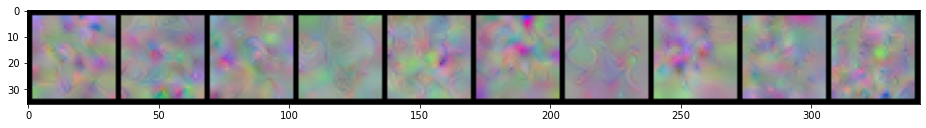
\includegraphics[width=\textwidth]{figures/INVERSION_CIFAR10_NN_0.png}



% \documentclass{article}
% \usepackage{graphicx}

% \ifluatex
%   \directlua{
%     tex.enableprimitives('', {'luaescapestring'})
%   }
%   \newcommand*{\Download}[2]{%
%     \IfFileExists{#1}{%
%     }{%
%       \directlua{
%         local io = require('io')
%         local http = require('socket.http')
%         local ltn12 = require('ltn12')
%         local file_name = '\luaescapestring{#1}'
%         local url = '\luaescapestring{#2}'
%         texio.write_nl('Downloading: ' .. file_name)
%         texio.write_nl('')
%         http.request{
%           url=url,
%           sink=ltn12.sink.file(io.open(file_name, 'w'))
%         }
%       }%
%     }%
%     \edef\DownloadFile{#1}%
%   }
% \else
%   \newcommand*{\Download}[2]{%
%     \IfFileExists{#1}{%
%     }{%
%       \immediate\write18{%
%         wget -O "#2" "#1"%
%       }%
%     }%
%     \edef\DownloadFile{#1}%
%   }%
% \fi

% \begin{figure}
% \centering
% \Download{profile-pics-16.jpg}{%
%     https://cdn.mos.cms.futurecdn.net/42E9as7NaTaAi4A6JcuFwG-970-80.jpg%
% }
% \includegraphics{\DownloadFile}
% \end{figure}
% \section{Results}

\subsection{Quantitative Results}

\pgfplotstableset{
col sep = comma,
string replace*={_}{\textsubscript},
every head row/.style={before row=\toprule,after row=\midrule},
every last row/.style={after row=\bottomrule},
every column/.style={column type=l, precision=1, zerofill},
columns={[index]0, [index]1, [index]2, [index]3, [index]4, [index]5, [index]6},
display columns/0/.style={column name=\textbf{Method}, column type=l, string type},
display columns/1/.style={column name=\textbf{Accuracy} [\%], multiply with=100},
display columns/2/.style={column name=\makecell{validation \\ \textbf{Accuracy}} [\%], column type=l, multiply with=100},
display columns/3/.style={column name=\makecell{verifier \\ \textbf{Accuracy}} [\%], column type=l, multiply with=100},
display columns/4/.style={column name=\textbf{l2-error}},
display columns/5/.style={column name=\textbf{PSNR}},
display columns/6/.style={column name=\textbf{SSIM} [\%], column type=l, multiply with=100},
}
\pgfplotstabletypeset{figures/reconstruction_CIFAR10_baseline.csv}
\pgfplotstabletypeset{figures/reconstruction_CIFAR10_results.csv}


% \chapter{Introduction}

\label{Introduction}

Neural networks designed for a classification task typically map inputs coming from a very high-dimensional space to a rather low-dimensional space - the space of possible classes.
$$
x \in \R^n,\ y \in \R^m ,\ n \gg m
$$
$$\phi (x) = y
$$
Given the nature of such a task, this forward process typically incurs in a huge loss of information. When $n > m$ and the data is not contained in some lower-dimensional submanifold, then the restriction of the map $\phi$ to the data manifold can not be bijective and therefore not invertible. 
Thus, given only the output, it is generally not possible to recover the input.
Typically, this transformation of the input to more abstract, meaningful features, along with the resulting compression is desired. Yet, the inverse problem of accurately modeling the posterior distribution $p(x|\;y)$ or an approximation thereof is an active area of research with many applications.
Such advantages of invertibility can be more efficient training, knowledge distillation in teacher-student networks, but also most notably, interpretability of a neural network's decision process - a big concern in security-related fields such as medical sciences, autonomous vehicles and face-recognition. 

Some recent work in this area are \textit{Invertible Neural Networks} \citep{ardizzone2018analyzing} , \textit{Glow: Generative Flow with Invertible 1x1 Convolutions} \citep{kingma2018glow} and \textit{Invertible Residual Networks} \citep{behrmann2018invertible}. The methods used vary from noise-optimization, direct parametrization to solving fixed-point iterations.

For the sake of interpretability, it is often enough to be able to sample from the posterior distribution.
The method that will be further examined in this work is an iterative refinement-process that optimizes random noise or an existing image to meet some criterion. This method was made popular by the computer vision program \textit{DeepDream} \citep{DeepDream} and later further improved on by \textit{DeepInversion} \citep{DeepInversion}.

% \include{Chapters/Chapter1}
% % Chapter Template

\chapter{Feature Regularization} % Main chapter title

\label{Chapter2} % Change X to a consecutive number; for referencing this chapter elsewhere, use \ref{ChapterX}

%----------------------------------------------------------------------------------------
%	SECTION 1
%----------------------------------------------------------------------------------------

The basic idea used for dataset-reconstruction will be illustrated using a neural network trained for a simple classification task on a two-dimensional toy dataset. The same principle can be applied to image-classification networks, although intuition does not always hold in the very high-dimensional setting.

\begin{figure}
\centering
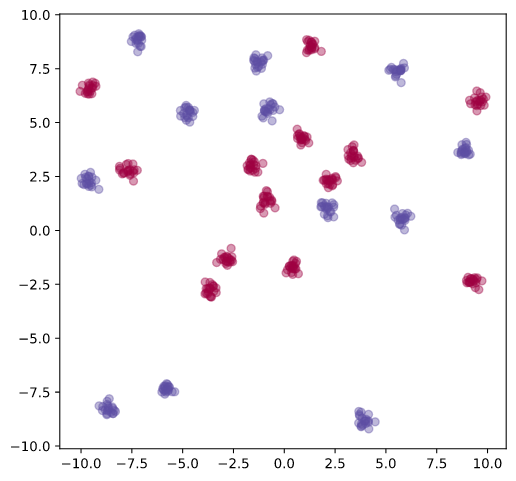
\includegraphics[width=0.5\textwidth]{Figures/toy_dataset.png}
\decoRule
\caption{toy dataset}
\label{fig:toy_dataset}
\end{figure}

%Given a dataset consisting of multiple classes, each with distinct features (as seen in \ref{fig:toy_dataset}), a neural network designed for the task of classification can generally (given that the  network is expressive enough) be trained to attain a high accuracy for this task.

\begin{figure}
\centering
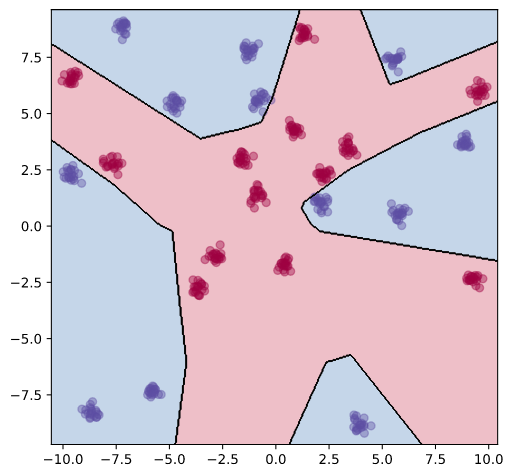
\includegraphics[width=0.5\textwidth]{Figures/toy_dataset_contour.png}
\decoRule
\caption{prediction by the neural network}
\label{fig:toy_dataset_contour}
\end{figure}

In the case of a two-dimensional dataset (as seen in \ref{fig:toy_dataset}), the predicted outcome of the neural network for any given point and the decision boundary can easily be visualized, as shown in \ref{fig:toy_dataset_contour}.
Here, a fully-connected neural network with two hidden layers of dimensions 8 and 6 was trained using the cross-entropy loss function to achieve a 100\% correct classification rate.

A method for reconstructing a data-point of a certain target-class $\hat y$, given only the neural network, is to start with a randomly initialized point in the input-space and then incrementally tweak it to maximize the neural network's response for the given class $\hat y$. In the same fashion as updating the weights of the network by gradient descent to minimize the error, the point can be updated instead to reach a lower classification-error.
This corresponds to minimizing the loss $\mathcal L$, given $\hat y$  with respect to the input $x$.
$$\min_x \mathcal L (x,\hat y)
$$

\begin{figure}
\centering
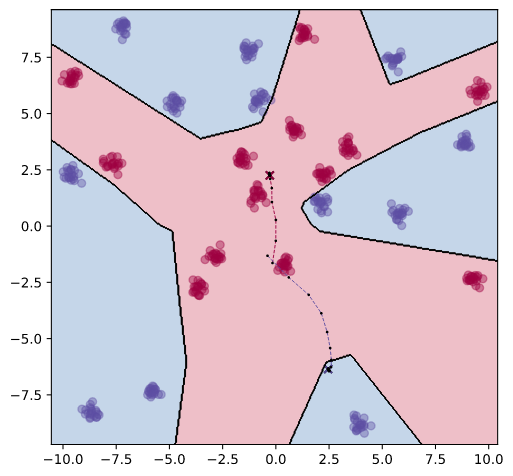
\includegraphics[width=0.5\textwidth]{Figures/toy_dataset_invert.png}
\decoRule
\caption{dataset-reconstruction}
\label{fig:toy_dataset_invert}
\end{figure}

The path such a data point might undertake in the optimization-process is shown in \ref{fig:toy_dataset_invert}.
In this setting, in order to gain further insight, the loss that is being optimized for can be plotted for each class individually. The resulting scalar-field is shown in  \ref{fig:toy_dataset_loss_landscape} and will be referred to as the \textit{loss-landscape}.

\begin{figure}
\centering
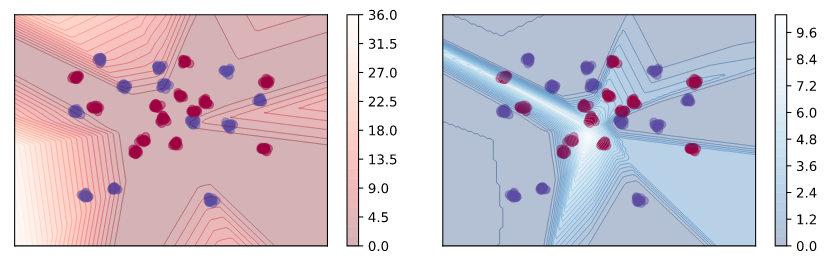
\includegraphics[width=\textwidth]{Figures/toy_dataset_loss_landscape.png}
\decoRule
\caption{loss-landscape}
\label{fig:toy_dataset_loss_landscape}
\end{figure}

Through this visualization it becomes clear that the points in \ref{fig:toy_dataset_invert} are moving toward local minima in the loss-landscape.
Some issues that are already foreseeable with this method is that the resulting end-points can (and in the most cases will) be chaotic with respect to the initialization. Points that are initially "close" can result in very different outcomes. It is also not immediately clear how many iteration-steps to perform or what criterion for stopping to meet when reconstruction is performed.
Another problem could be that points might "trail off" from the dataset-cluster or that points starting further away might keep their distance during the optimization-process. These points might be given a high score for belonging to the target-class by the network, yet they might not share the same statistics as "natural" data-points. This is seen in \ref{fig:toy_dataset_invert} as the reconstructed points don't end up near the clusters.

A way to combat this is to enforce similar statistics as those of the original dataset by including a regularization-term $\mathcal R$. In order to perform this, statistics, such as the mean and variance need to be tracked as additional parameters of the network (this can be done during training-time or once after training).
The statistics can be recorded for the whole dataset or for each class individually.
\cite{DeepInversion} have shown that using the statistics (mean and variance) stored in the batch-norm-layers of residual-networks can already greatly improve the reconstruction quality of images.
The advantage here is that these statistics are already included in a highly-utilized framework and are readily available without further labor. 

In the simple case of the toy-dataset, $\mathcal R$ could be formulated as
$$\mathcal R(x,\hat y) := \|x-\bar x_{\hat y}\|_2^2
\comma$$
where $\bar x_{\hat y}$ is the mean of class $\hat y$. Here, the variance has been omitted for simplicity.

\begin{figure}
\centering
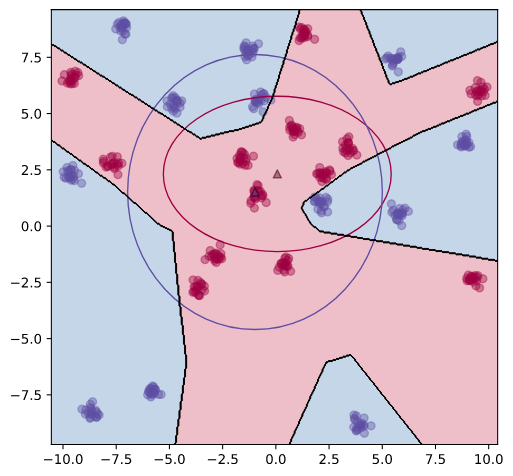
\includegraphics[width=0.5\textwidth]{Figures/toy_dataset_stats.png}
\decoRule
\caption{class-specific mean and variance}
\label{fig:toy_dataset_stats}
\end{figure}

Again, the effect of the additional regularization-term for each class can be made visible by plotting the resulting loss-landscape of $\mathcal R$, as seen in \ref{fig:toy_dataset_loss_stats}, which should reflect the class-dependent statistics.
\XXX{You used variance statistics for plotting}

\begin{figure}
\centering
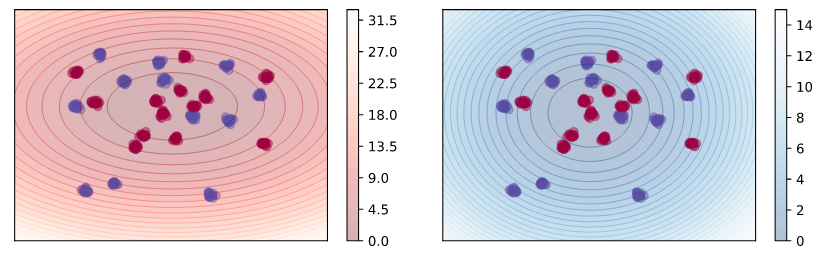
\includegraphics[width=\textwidth]{Figures/toy_dataset_loss_stats.png}
\decoRule
\caption{loss-landscape of the class-dependent regularization-term}
\label{fig:toy_dataset_loss_stats}
\end{figure}

The regularization may be incorporated in the loss by simply adding the new term (multiplied by a factor) to the original loss-formulation.
$$\min_x \mathcal L (x,\hat y) + \mathcal R(x,\hat y)
$$
The loss-landscape of the combination is shown in \ref{fig:toy_dataset_loss_combined}.

\begin{figure}
\centering
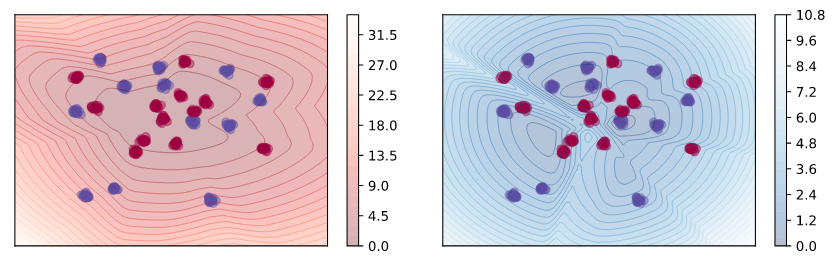
\includegraphics[width=\textwidth]{Figures/toy_dataset_loss_combined.png}
\decoRule
\caption{combined loss-landscape}
\label{fig:toy_dataset_loss_combined}
\end{figure}

So far, only the class-dependent statistics of the dataset have been taken into account. These statistics can be viewed as the statistics of the input to the first hidden layer of the neural network. In the same manner, the statistics of the input to subsequent layers of the network can be tracked and included in the regularization-term with an individual weighting.
$$\mathcal R(x,\hat y) := 
\lambda_0 \|x-\bar x_{\hat y}\|^2 
+ \lambda_1 \|\phi^{(1)} (x)-\bar x_{\hat y}^{(1)}\|^2
+ \lambda_2 \|\phi^{(2)} (x)-\bar x_{\hat y}^{(2)}\|^2
+ \ldots
\comma$$

where $\phi^{(i)}$ is the network's output of the $i$-th hidden layer and $\bar x_{\hat y}^{(i)}$ is the mean of $\phi^{(i)}$ over the data of the target-class $\hat y$.

$$\mathcal R(x,\hat y) := 
\sum_{i=0}^L \lambda_i \|\phi^{(i)} (x)-\bar x_{\hat y}^{(i)}\|^2
\comma$$
for a network with $L$ hidden layers, and where $\phi^{(0)}(x) := x$ and $\bar x_{\hat y}^{(0)} := \bar x_{\hat y}$.
$\lambda_i$ are seen as additional hyper-parameters.

%%-----------------------------------
%%	SUBSECTION 1
%%-----------------------------------
%\subsection{Subsection 1}
%
%
%
%%-----------------------------------
%%	SUBSECTION 2
%%-----------------------------------
%
%\subsection{Subsection 2}
%
%%----------------------------------------------------------------------------------------
%%	SECTION 2
%%----------------------------------------------------------------------------------------
%
%\section{Main Section 2}
 
% \include{Chapters/Chapter3}
% \include{Chapters/Chapter4} 
% \include{Chapters/Chapter5} 

%----------------------------------------------------------------------------------------
%	THESIS CONTENT - APPENDICES
%----------------------------------------------------------------------------------------

\appendix % Cue to tell LaTeX that the following "chapters" are Appendices

% Include the appendices of the thesis as separate files from the Appendices folder
% Uncomment the lines as you write the Appendices

% % Appendix Template

\chapter{Implementation Details} % Main appendix title

\label{AppendixA} % Change X to a consecutive letter; for referencing this appendix elsewhere, use \ref{AppendixX}

Details of implementation...
%\chapter{Results}
\label{AppendixImages}



\begin{figure}
    % \centerline{
    % \hspace*{6mm}
    % \begin{minipage}{0.6\textwidth}
    % 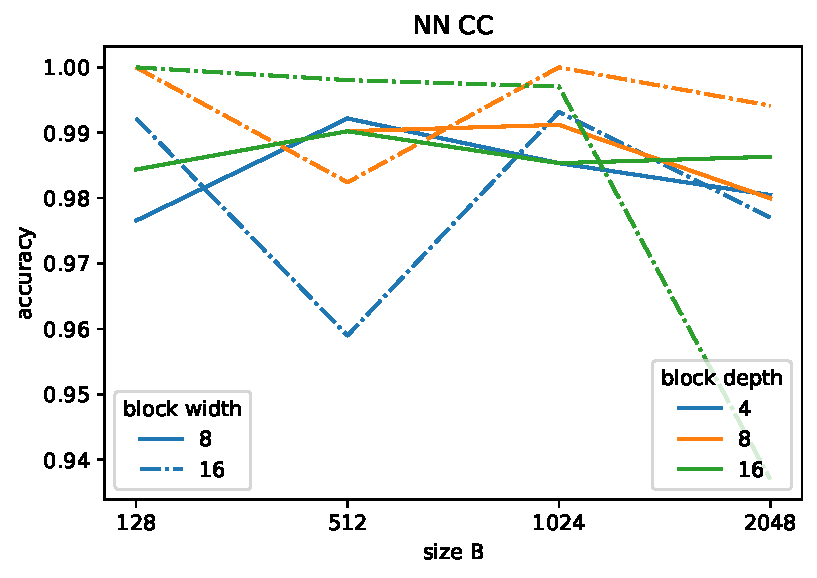
\includegraphics[width=\textwidth]{figures/comparison_CIFAR10_accuracy_NN_CC.pdf}
    % \end{minipage}%
    % \begin{minipage}{0.6\textwidth}
    % 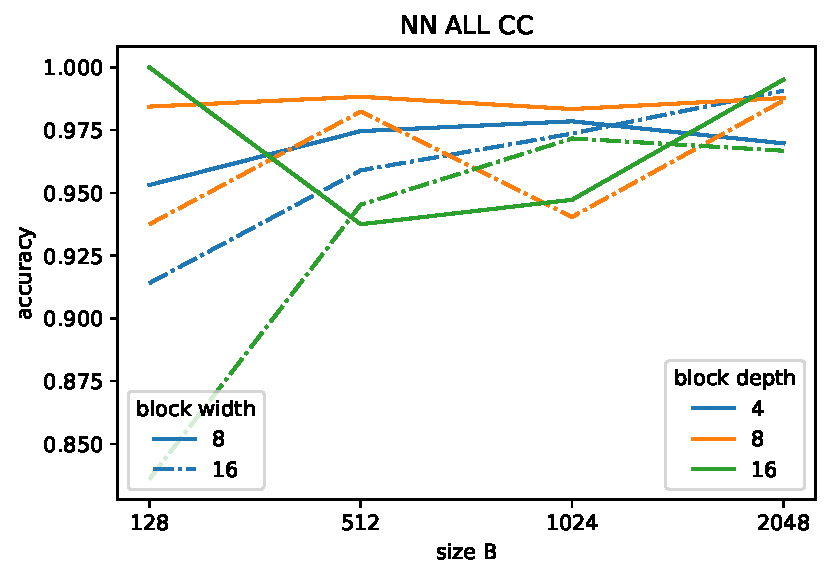
\includegraphics[width=\textwidth]{figures/comparison_CIFAR10_accuracy_NN_ALL_CC.pdf}
    % \end{minipage}
    % }
    \centerline{
    \hspace*{6mm}
    \begin{minipage}{0.6\textwidth}
    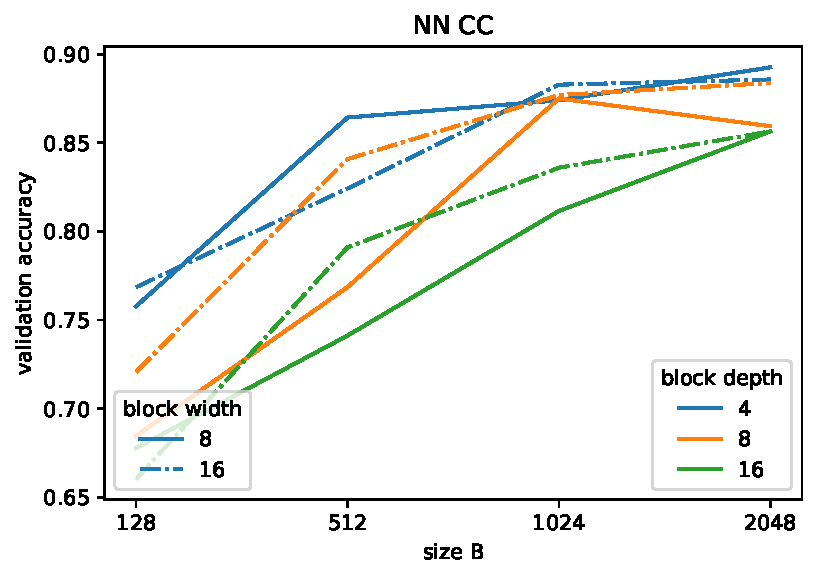
\includegraphics[width=\textwidth]{figures/comparison_CIFAR10_validation_accuracy_NN_CC.pdf}
    \end{minipage}%
    \begin{minipage}{0.6\textwidth}
    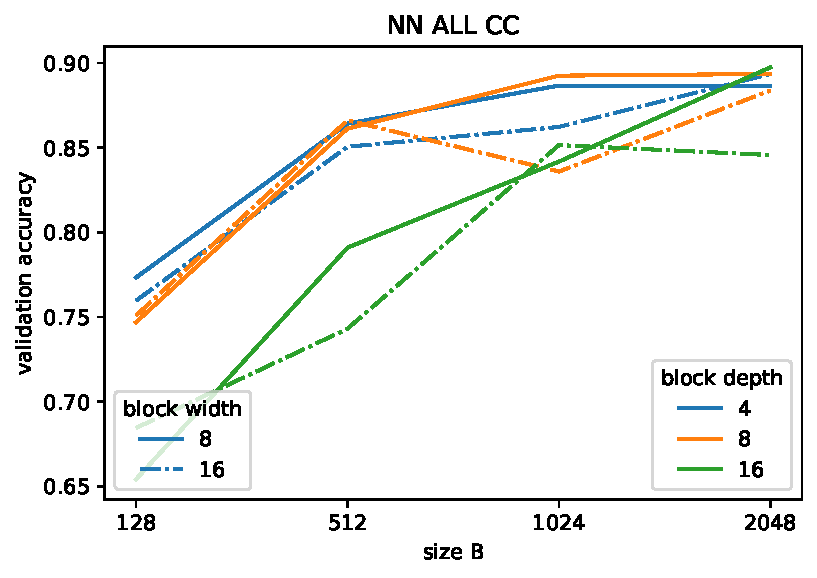
\includegraphics[width=\textwidth]{figures/comparison_CIFAR10_validation_accuracy_NN_ALL_CC.pdf}
    \end{minipage}
    }
    \centerline{
    \hspace*{6mm}
    \begin{minipage}{0.6\textwidth}
    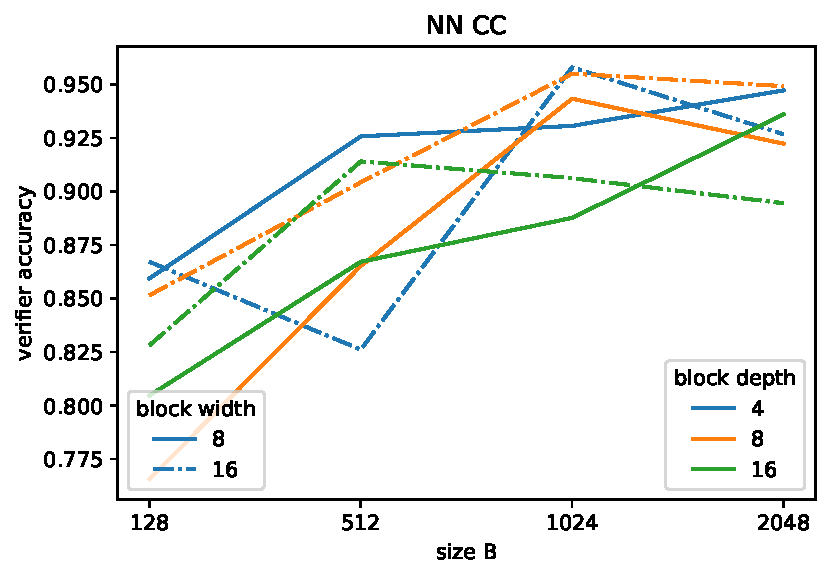
\includegraphics[width=\textwidth]{figures/comparison_CIFAR10_verifier_accuracy_NN_CC.pdf}
    \end{minipage}%
    \begin{minipage}{0.6\textwidth}
    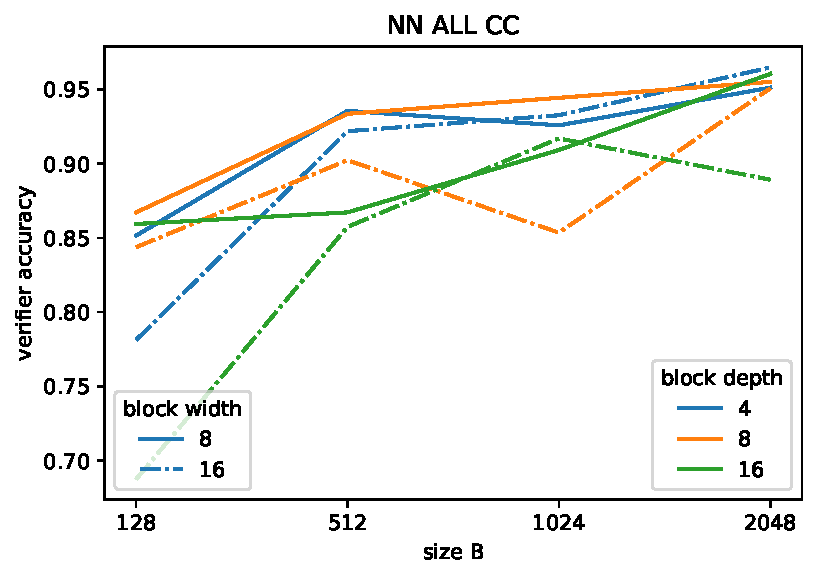
\includegraphics[width=\textwidth]{figures/comparison_CIFAR10_verifier_accuracy_NN_ALL_CC.pdf}
    \end{minipage}
    }
    \centerline{
    \hspace*{6mm}
    \begin{minipage}{0.6\textwidth}
    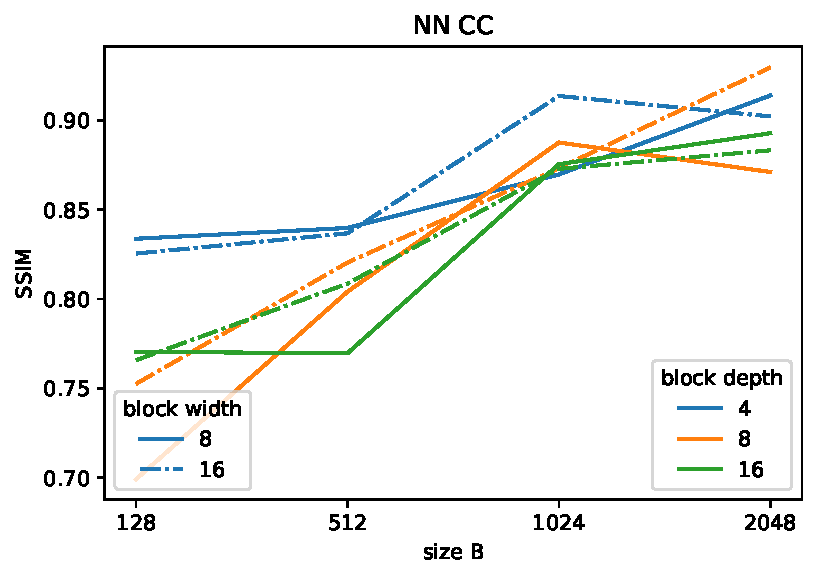
\includegraphics[width=\textwidth]{figures/comparison_CIFAR10_SSIM_NN_CC.pdf}
    \end{minipage}%
    \begin{minipage}{0.6\textwidth}
    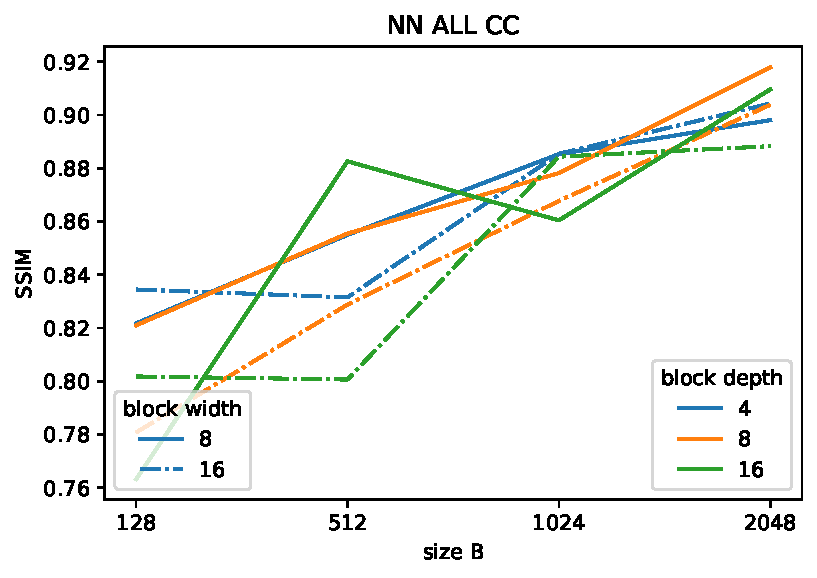
\includegraphics[width=\textwidth]{figures/comparison_CIFAR10_SSIM_NN_ALL_CC.pdf}
    \end{minipage}
    }
    \caption{Hyperparameter influence on metrics}
    \label{fig:HyperparamInfluence}
\end{figure}



% \begin{figure}
%     \setlength{\abovecaptionskip}{0pt plus 0pt minus 0pt}
%     \setlength{\belowcaptionskip}{16pt plus 0pt minus 0pt}
%     \caption*{\normalsize{\textit{Ground Truth}}}
%     \centerline{\hspace*{8mm}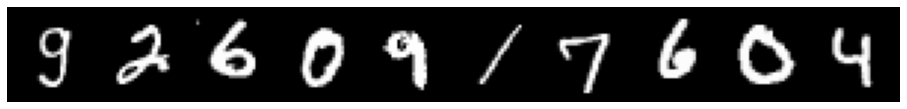
\includegraphics[width=1.4\textwidth]{figures/reconstruction_MNIST_ground_truth.png}}
%     \caption*{\normalsize{\textit{Distorted}}}
%     \centerline{\hspace*{8mm}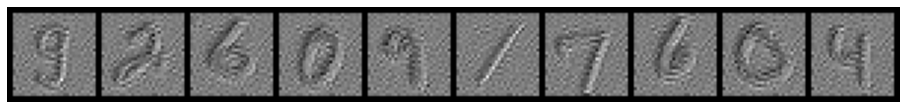
\includegraphics[width=1.4\textwidth]{figures/reconstruction_MNIST_distorted.png}}
%     \caption*{\normalsize{CRITERION}}
%     \centerline{\hspace*{8mm}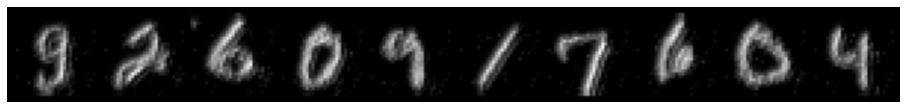
\includegraphics[width=1.4\textwidth]{figures/reconstruction_MNIST_CRITERION_epoch_100.png}}
%     \caption*{\normalsize{NN}}
%     \centerline{\hspace*{8mm}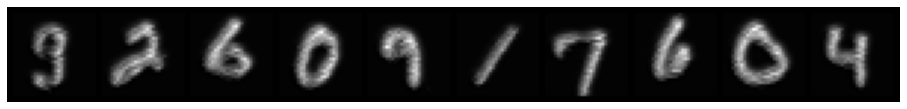
\includegraphics[width=1.4\textwidth]{figures/reconstruction_MNIST_NN_epoch_100.png}}
%     \caption*{\normalsize{NN CC}}
%     \centerline{\hspace*{8mm}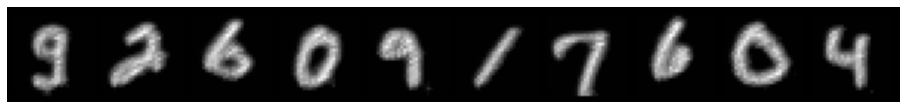
\includegraphics[width=1.4\textwidth]{figures/reconstruction_MNIST_NN_CC_epoch_100.png}}
%     \caption*{\normalsize{NN ALL}}
%     \centerline{\hspace*{8mm}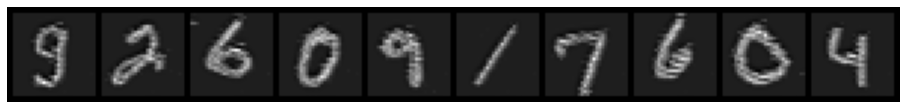
\includegraphics[width=1.4\textwidth]{figures/reconstruction_MNIST_NN_ALL_epoch_100.png}}
%     \caption*{\normalsize{NN ALL CC}}
%     \centerline{\hspace*{8mm}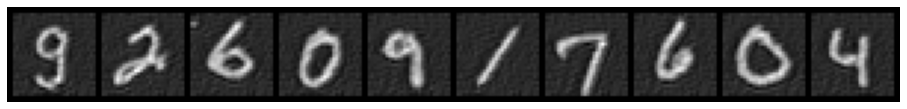
\includegraphics[width=1.4\textwidth]{figures/reconstruction_MNIST_NN_ALL_CC_epoch_100.png}}
%     \label{fig:MNIST_Images}
% \end{figure}
% \begin{figure}
%     \setlength{\abovecaptionskip}{0pt plus 0pt minus 0pt}
%     \setlength{\belowcaptionskip}{16pt plus 0pt minus 0pt}
%     \caption*{\normalsize{RANDOM NN}}
%     \centerline{\hspace*{8mm}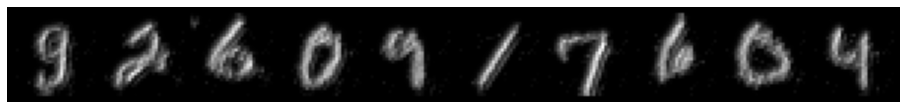
\includegraphics[width=1.4\textwidth]{figures/reconstruction_MNIST_RANDOM_NN_epoch_100.png}}
%     \caption*{\normalsize{RANDOM NN CC}}
%     \centerline{\hspace*{8mm}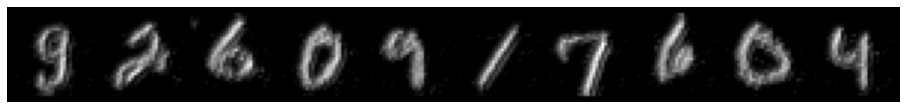
\includegraphics[width=1.4\textwidth]{figures/reconstruction_MNIST_RANDOM_NN_CC_epoch_100.png}}
%     \caption*{\normalsize{RP}}
%     \centerline{\hspace*{8mm}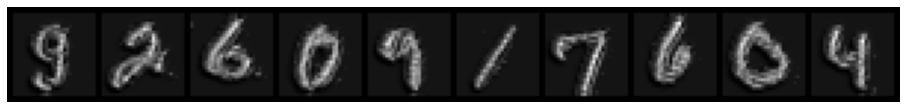
\includegraphics[width=1.4\textwidth]{figures/reconstruction_MNIST_RP_epoch_100.png}}
%     \caption*{\normalsize{RP CC}}
%     \centerline{\hspace*{8mm}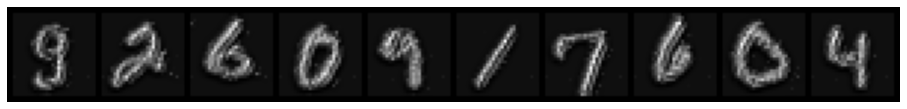
\includegraphics[width=1.4\textwidth]{figures/reconstruction_MNIST_RP_CC_epoch_100.png}}
%     \caption*{\normalsize{RP ReLU}}
%     \centerline{\hspace*{8mm}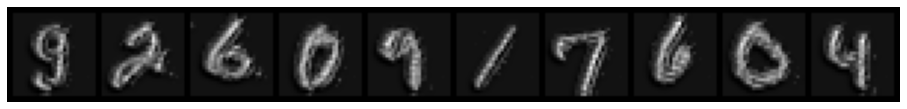
\includegraphics[width=1.4\textwidth]{figures/reconstruction_MNIST_RP_ReLU_epoch_100.png}}
%     \caption*{\normalsize{RP ReLU CC}}
%     \centerline{\hspace*{8mm}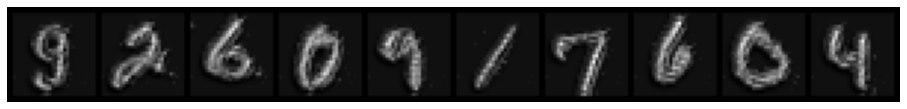
\includegraphics[width=1.4\textwidth]{figures/reconstruction_MNIST_RP_ReLU_CC_epoch_100.png}}
%     \caption*{\normalsize{COMBINED CC}}
%     \centerline{\hspace*{8mm}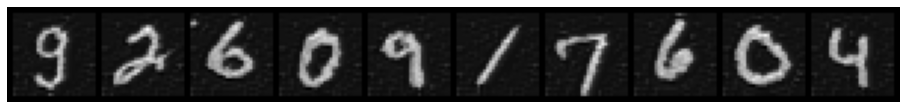
\includegraphics[width=1.4\textwidth]{figures/reconstruction_MNIST_COMBINED_CC_epoch_100.png}}
% \end{figure}




\begin{figure}
    \centering
    \setlength{\abovecaptionskip}{0pt plus 0pt minus 0pt}
    \setlength{\belowcaptionskip}{16pt plus 0pt minus 0pt}
    \caption*{\normalsize{\textit{Ground Truth}}}
    \rule{0.4\textwidth}{.4pt}
    
    \centerline{\hspace*{8mm}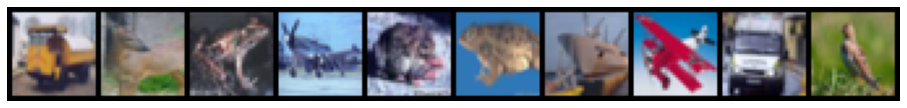
\includegraphics[width=1.4\textwidth]{figures/reconstruction_CIFAR10_ground_truth.png}}
    \caption*{\normalsize{\textit{Distorted}}}
    \rule{0.4\textwidth}{.4pt}
    
    \centerline{\hspace*{8mm}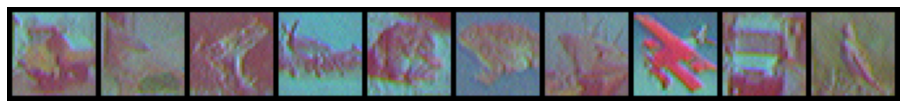
\includegraphics[width=1.4\textwidth]{figures/reconstruction_CIFAR10_distorted.png}}
    \caption*{\normalsize{CRITERION}}
    \rule{0.4\textwidth}{.4pt}
    
    \centerline{\hspace*{8mm}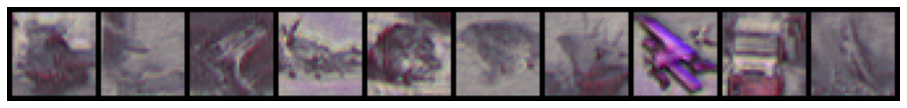
\includegraphics[width=1.4\textwidth]{figures/reconstruction_CIFAR10_CRITERION_epoch_100.png}}
    \caption*{\normalsize{NN}}
    \rule{0.4\textwidth}{.4pt}
    
    \centerline{\hspace*{8mm}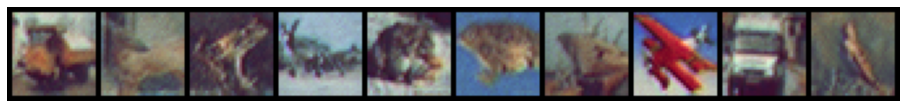
\includegraphics[width=1.4\textwidth]{figures/reconstruction_CIFAR10_NN_epoch_100.png}}
    \caption*{\normalsize{NN CC}}
    \rule{0.4\textwidth}{.4pt}
    
    \centerline{\hspace*{8mm}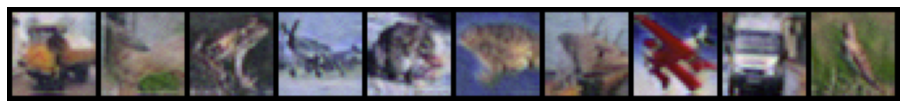
\includegraphics[width=1.4\textwidth]{figures/reconstruction_CIFAR10_NN_CC_epoch_100.png}}
    \caption*{\normalsize{NN ALL}}
    \rule{0.4\textwidth}{.4pt}
    
    \centerline{\hspace*{8mm}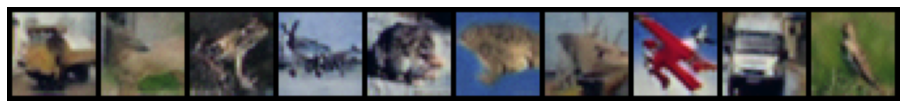
\includegraphics[width=1.4\textwidth]{figures/reconstruction_CIFAR10_NN_ALL_epoch_100.png}}
    \caption*{\normalsize{NN ALL CC}}
    \rule{0.4\textwidth}{.4pt}
    
    \centerline{\hspace*{8mm}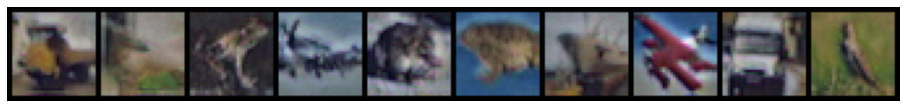
\includegraphics[width=1.4\textwidth]{figures/reconstruction_CIFAR10_NN_ALL_CC_epoch_100.png}}
\end{figure}

\begin{figure}
    \centering
    \setlength{\abovecaptionskip}{0pt plus 0pt minus 0pt}
    \setlength{\belowcaptionskip}{16pt plus 0pt minus 0pt}
    \caption*{\normalsize{RANDOM NN}}
    \rule{0.4\textwidth}{.4pt}
    
    \centerline{\hspace*{8mm}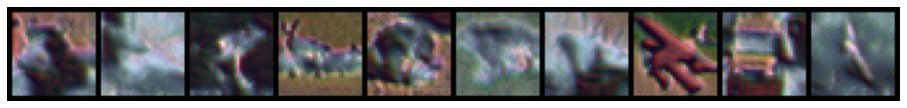
\includegraphics[width=1.4\textwidth]{figures/reconstruction_CIFAR10_RANDOM_NN_epoch_100.png}}
    \caption*{\normalsize{RANDOM NN CC}}
    \rule{0.4\textwidth}{.4pt}
    
    \centerline{\hspace*{8mm}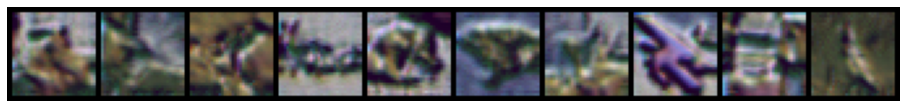
\includegraphics[width=1.4\textwidth]{figures/reconstruction_CIFAR10_RANDOM_NN_CC_epoch_100.png}}
    \caption*{\normalsize{RP}}
    \rule{0.4\textwidth}{.4pt}
    
    \centerline{\hspace*{8mm}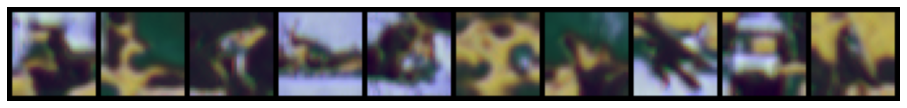
\includegraphics[width=1.4\textwidth]{figures/reconstruction_CIFAR10_RP_epoch_100.png}}
    \caption*{\normalsize{RP CC}}
    \rule{0.4\textwidth}{.4pt}
    
    \centerline{\hspace*{8mm}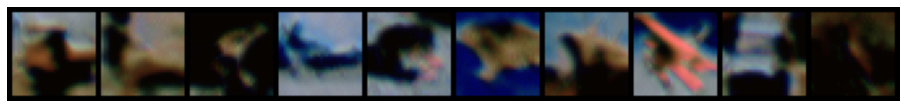
\includegraphics[width=1.4\textwidth]{figures/reconstruction_CIFAR10_RP_CC_epoch_100.png}}
    \caption*{\normalsize{RP ReLU}}
    \rule{0.4\textwidth}{.4pt}
    
    \centerline{\hspace*{8mm}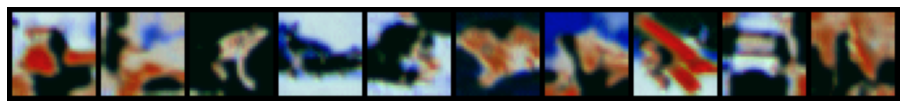
\includegraphics[width=1.4\textwidth]{figures/reconstruction_CIFAR10_RP_ReLU_epoch_100.png}}
    \caption*{\normalsize{RP ReLU CC}}
    \rule{0.4\textwidth}{.4pt}
    
    \centerline{\hspace*{8mm}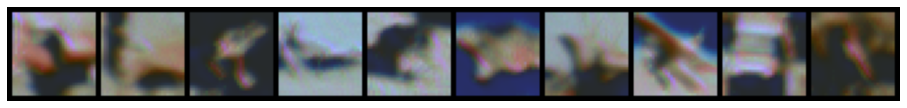
\includegraphics[width=1.4\textwidth]{figures/reconstruction_CIFAR10_RP_ReLU_CC_epoch_100.png}}
    \caption*{\normalsize{COMBINED CC}}
    \rule{0.4\textwidth}{.4pt}
    
    \centerline{\hspace*{8mm}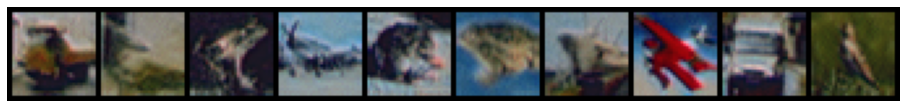
\includegraphics[width=1.4\textwidth]{figures/reconstruction_CIFAR10_COMBINED_CC_epoch_100.png}}
\end{figure}





%\include{Appendices/AppendixC}

%----------------------------------------------------------------------------------------
%	BIBLIOGRAPHY
%----------------------------------------------------------------------------------------

\printbibliography[heading=bibintoc]

%----------------------------------------------------------------------------------------

\end{document}  
